\documentclass{ximera}

\usepackage{float}

\newcommand{\R}{\mathbb R}

\newcommand{\href}[2]{#2\footnote{\url{#1}}}
\newcommand{\verticalvector}[1]{\begin{bmatrix}#1\end{bmatrix}}
\newcommand{\gt}{>}

\pgfplotsset{compat=1.8}
\graphicspath{
{./}
{introduction/}
{unit1/}
{unit1/theGeometryOfLinearEquations/}
{unit1/EliminationwithMatrices/}
{unit1/MultiplicationandInverseMatrices/}
}


\title{The Geometry of Linear Equations}

\begin{document}
\begin{abstract}
  Unit 1 MIT OCW Linear Algebra: The Geometry of Linear Equations
\end{abstract}
\maketitle

The MIT OCW Video Lecture can be found
here:\video{https://www.youtube.com/watch?v=ZK3O402wf1c}


A major application of linear algebra is to solving systems of linear
equations. This lecture presents three ways of thinking about these
systems. The ``row method'' focuses on the individual equations, the
``column method'' focuses on combining the columns, and the ``matrix
method'' is an even more compact and powerful way of describing
systems of linear equations.

\begin{figure}[H]
\begin{image}
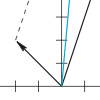
\includegraphics{1_1.jpg}
\end{image}
\caption{Portion of Fig. 2.2 from the textbook \textit{Introduction to
    Linear Algebra}.}
\end{figure}

The fundamental problem of linear algebra is to solve $n$ linear
equations in $n$ unknowns; for example:
\begin{align*}
  2x-y &= 0 \\ 
  -x+2y &= 3
\end{align*}
The system above is two dimensional ($n = 2$). By adding a third
variable $z$ we could expand it to three dimensions.

In this first lecture on linear algebra we view this problem in three
ways:

\begin{itemize}
\item Row Picture
\item Column Picture
\item Matrix Picture
\end{itemize}

\section*{Row Picture}

Plot the points that satisfy each equation. The intersection of the
plots (if they do intersect) represents the solution to the system of
equations. Looking at Figure~\ref{fig:intplot} we see that the
solution to this system of equations is $x = 1$, $y = 2$.

\begin{figure}[H]\label{fig:intplot}
\begin{image}
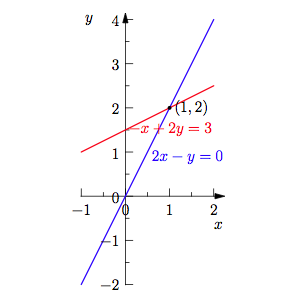
\includegraphics{Geometry1.png}
\end{image}
\caption{The lines $2x - y = 0$ and $-x + 2y = 3$ intersect at the
  point $(1, 2)$}
\end{figure}

We plug this solution in to the original system of equations to check
our work:

\begin{align*}
2\cdot1-2 &= 0\\
-1+2\cdot2 &= 3
\end{align*}
The solution to a three dimensional system of equations is the common
point of intersection of three planes (if there is one).

\section*{Column Picture}

In the column picture we rewrite the system of linear equations as a
single equation by turning the coefficients in the columns of the
system into vectors:
\[
x\verticalvector{\phantom{-} 2\\-1} + y\verticalvector{-1\\\phantom{-}
  2} = \verticalvector{0\\3}
\]
Given two vectors $\mathbf{c}$ and $\mathbf{d}$ and scalars $x$ and
$y$, the sum $x\mathbf{c} + y\mathbf{d}$ is called a linear
combination of $\mathbf{c}$ and $\mathbf{d}$. Linear combinations are
important throughout this course.


Geometrically, we want to find numbers x and y so that x copies of
vector $\verticalvector{\phantom{-}2\\-1}$ added to y copies of vector
$\verticalvector{-1\\\phantom{-}2}$ equals to vector
$\verticalvector{0\\3}$. As we see from Figure~\ref{fig:rowpict}, $x =
1$ and $y = 2$, agreeing with the row picture in
Figure~\ref{fig:rowpict}.

\begin{figure}[H]\label{fig:rowpict}
\begin{image}
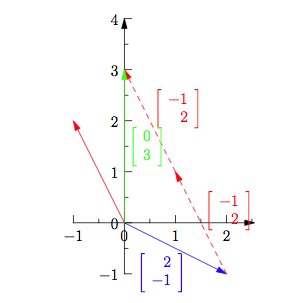
\includegraphics{Geometry2.png}
\end{image}
\caption{A linear combination of the column vectors equals the vector
  $\mathbf{b}$.}
\end{figure}

In three dimensions, the column picture requires us to find a linear
combinations of three 3-dimensional vectors that equals the vector $b$.

\section*{Matrix Picture}

We write the system of equations
\begin{align*}
2x-y = 0\\
-x+2y = 3
\end{align*}
as a single equation by using matrices and vectors:
\[
\begin{bmatrix} \phantom{-}2 & -1\\ -1 & \phantom{-}2 \end{bmatrix} \begin{bmatrix} 
  x\\y \end{bmatrix} =  \begin{bmatrix} 0\\3 \end{bmatrix}
\]
The matrix $A = \begin{bmatrix} \phantom{-}2 & -1\\-1 & \phantom{-}2 \end{bmatrix}$ 
is called the coefficient matrix. The vector $x = \begin{bmatrix} x\\y \end{bmatrix}$ 
is the vector of unknowns. The values on the right hand side of the equations form the 
vector \textbf{b}:
\begin{align*}
A\mathbf{x} = b.
\end{align*}

The three dimensional matrix picture is very like the two dimensional one, except 
that the vectors and matrices increase in size.

\subsection*{Matrix Multiplication}
How do we multiply a matrix A by a vector x?\\

\[\begin{bmatrix} 2 & 5\\ 1 & 3 \end{bmatrix} \begin{bmatrix} 1\\2 \end{bmatrix} = ?\]\\

\noindent
One method is to think of the entries of x as the coefficients of a linear
combination of the column vectors of the matrix:
\[\begin{bmatrix} 2 & 5\\ 1 & 3 \end{bmatrix} \begin{bmatrix} 1\\2 
\end{bmatrix} = 1\begin{bmatrix} 2\\1 \end{bmatrix} + 2 
\begin{bmatrix} 5\\3 \end{bmatrix} = \begin{bmatrix} 12\\7 \end{bmatrix}\]\\
This technique shows that Ax is a linear combination of the columns of A. 
You may also calculate the product Ax by taking the dot product of each 
row of A with the vector x:
\[\begin{bmatrix} 2 & 5\\ 1 & 3 \end{bmatrix} \begin{bmatrix} 1\\2 \end{bmatrix} 
= \begin{bmatrix} 2 \cdot 1 + 5 \cdot 2\\ 1 \cdot 1 + 3 \cdot 2 \end{bmatrix} = 
\begin{bmatrix} 12\\7 \end{bmatrix}\]

\subsection*{Linear Independence}

In the column and matrix pictures, the right hand side of the equation is a 
vector b. Given a matrix A, can we solve:
$A\mathbf{x} = b$
for every possible vector b? In other words, do the linear combinations of 
the column vectors fill the xy-plane (or space, in the three dimensional case)?

If the answer is "no", we say that A is a singular matrix. In this singular 
case its column vectors are linearly dependent; all linear combinations of 
those vectors lie on a point or line (in two dimensions) or on a point, line 
or plane (in three dimensions). The combinations don't fill the whole space.

\section*{Recitation}

\begin{question}
Problem is to solve:
\begin{align*}
2x+y = 3
x-2y = -1
\end{align*}
Solve Algebraically, then show its down and column picture

\begin{solution}
\begin{hint}
	Using the second equation solve for x
\end{hint}
\begin{hint}
	$x=2y-1$
\end{hint}
\begin{hint}
	Substituting x into the first equation gives $2(2y-1))+y=3$ which simplifies to $5y-2=3$ or $y=1$
\end{hint}
\begin{hint}
	now substituting y back into this equation $x=2y-1$ gives $x=2\cdot1-1 = 1$
\end{hint}
what are the values of x and y? $x = $ \answer(1)  $y= $ \answer(1)
\end{solution}

\end{question}

The MIT Recitation video for this question is here:
here:\video{https://www.youtube.com/watch?v=uNKDw46_Ev4}

\section*{Homework}
\begin{question}
1.3 problem 4 Introduction to Linear Algebra: Strang) Find a combination $x_1\mathbf{w_1} + x_2\mathbf{w_2} + x_3\mathbf{w_3}$ that gives the zero vector for the following vectors:
\begin{align*}
\mathbf{w_1} = \verticalvector{1\\2\\3} \mathbf{w_2} = \verticalvector{4\\5\\6} \mathbf{w_3} = \verticalvector{7\\8\\9}
\end{align*}
and are the vectors independent or dependent.
\begin{solution}
\begin{hint}
We might observe that $w_1 + w_3 -2w_2 = 0$, or we might simultaneously solve the system of equations.
\end{hint}
\begin{hint}
convert from the 3 vectors to a system of equations
\begin{align*}
1x_1+4x_2+7x_3=0\\
2x_1+5x_2+8x_3=0\\
3x_1+6x_2+9x_3=0\\
\end{align*}
\end{hint}
\begin{hint}
Subtracting twice equation 1 from equation 2 gives us $-3x_2 - 6x_3 = 0$. Subtracting thrice equation 1 from equation 3 gives us $-6x_2 - 12x_3 = 0$, which is equivalent to the previous equation and so leads us to suspect that the vectors are dependent. At this point we might guess $x_2 = -2$ and $x_3 = 1$ which would lead us to the answer we observed above:
\begin{align*}
x_1 =1, x_2 =-2, x_3 =1\\
\mathbf{w_1}-2\mathbf{w_2}+\mathbf{w_3} =0.
\end{align*}
Those vectors are dependent because there is a combination of the vectors
that gives the zero vector.
\end{hint}
\begin{hint}
The three vectors lie in a \textbf{plane}.
\end{hint}
What is the linear combination of the three vectors \answer{$w_1+w_3-2w_2=0$}.
Are the vectors independent or dependent?  \answer{dependent}.
So the three vectors lie in a \answer{Plane}. The matrix W with those columns
is not invertible.
\end{solution}
\end{question}

\begin{question}
Multiply the two matrices $A \cdot \mathbf{x}$:
\[\begin{bmatrix} 1&2&0\\2&0&3\\4&1&1 \end{bmatrix} \verticalvector{\phantom{-}3\\-2\\\phantom{-}1}\]

\begin{solution}
\begin{hint}
\[A \cdot \mathbf{x} = \verticalvector{1\cdot3+2\cdot(-2)+0\cdot1\\6+0+3\\12-2+1}\]
\end{hint}

\begin{hint}
\[A \cdot \mathbf{x} = \verticalvector{-1\\\phantom{-}9\\\phantom{-}11}\]
\end{hint}
\[\begin{bmatrix} 1&2&0\\2&0&3\\4&1&1 \end{bmatrix} \verticalvector{\phantom{-}3\\-2\\\phantom{-}1}\ = \begin{matrix-answer}[name=M]
      correctMatrix = [[''-1'],['9'],['11']]
    \end{matrix-answer}\]
\end{solution}
\end{question}

\begin{question}
\begin{solution}
\begin{hint}
\end{hint}
\end{solution}
\end{question}

\end{document}
